%File: formatting-instructions-latex-2024.tex
%release 2024.0
\documentclass[letterpaper]{article} % DO NOT CHANGE THIS
\usepackage{aaai24}
% \usepackage[submission]{aaai24}  % DO NOT CHANGE THIS
\usepackage{times}  % DO NOT CHANGE THIS
\usepackage{helvet}  % DO NOT CHANGE THIS
\usepackage{courier}  % DO NOT CHANGE THIS
\usepackage[hyphens]{url}  % DO NOT CHANGE THIS
\usepackage{graphicx} % DO NOT CHANGE THIS
\urlstyle{rm} % DO NOT CHANGE THIS
\def\UrlFont{\rm}  % DO NOT CHANGE THIS
\usepackage{natbib}  % DO NOT CHANGE THIS AND DO NOT ADD ANY OPTIONS TO IT
\usepackage{caption} % DO NOT CHANGE THIS AND DO NOT ADD ANY OPTIONS TO IT
\frenchspacing  % DO NOT CHANGE THIS
\setlength{\pdfpagewidth}{8.5in}  % DO NOT CHANGE THIS
\setlength{\pdfpageheight}{11in}  % DO NOT CHANGE THIS
%
% These are recommended to typeset algorithms but not required. See the subsubsection on algorithms. Remove them if you don't have algorithms in your paper.
\usepackage{algorithm}
\usepackage{algorithmic}

%
% These are are recommended to typeset listings but not required. See the subsubsection on listing. Remove this block if you don't have listings in your paper.
\usepackage{newfloat}
\usepackage{listings}
\DeclareCaptionStyle{ruled}{labelfont=normalfont,labelsep=colon,strut=off} % DO NOT CHANGE THIS
\lstset{%
	basicstyle={\footnotesize\ttfamily},% footnotesize acceptable for monospace
	numbers=left,numberstyle=\footnotesize,xleftmargin=2em,% show line numbers, remove this entire line if you don't want the numbers.
	aboveskip=0pt,belowskip=0pt,%
	showstringspaces=false,tabsize=2,breaklines=true}
\floatstyle{ruled}
\newfloat{listing}{tb}{lst}{}
\floatname{listing}{Listing}

% Keep the \pdfinfo as shown here. There's no need
% for you to add the /Title and /Author tags.
\pdfinfo{
/TemplateVersion (2024.1)
}


%%% My packages %%%
\usepackage{amsmath}
\usepackage{amssymb}
\usepackage{booktabs}
\usepackage{array}
\usepackage{soul}
\usepackage{multirow}
\usepackage{subcaption}
\captionsetup{font=small}
\captionsetup[sub]{font=small}

\usepackage{xcolor}
\newcommand\kso[1]{{\textcolor{magenta}{#1}}}

\usepackage{pifont}
\newcommand{\cmark}{\ding{51}}
\newcommand{\xmark}{\ding{55}}

\renewcommand{\paragraph}[1]{
     \noindent{\textbf{#1}} 
 }
 
% for Korean
\usepackage{kotex}
% \usepackage[cjk]{kotex}

% Support for easy cross-referencing 
\usepackage[capitalize]{cleveref}
\crefname{section}{Sec.}{Secs.}
\Crefname{section}{Section}{Sections}
\Crefname{table}{Table}{Tables}
\crefname{table}{Tab.}{Tabs.}

\newcommand{\etal}{\textit{et al}. }
\newcommand{\ie}{\textit{i}.\textit{e}., }
\newcommand{\eg}{\textit{e}.\textit{g}., }

% DISALLOWED PACKAGES
% \usepackage{authblk} -- This package is specifically forbidden
% \usepackage{balance} -- This package is specifically forbidden
% \usepackage{color (if used in text)
% \usepackage{CJK} -- This package is specifically forbidden
% \usepackage{float} -- This package is specifically forbidden
% \usepackage{flushend} -- This package is specifically forbidden
% \usepackage{fontenc} -- This package is specifically forbidden
% \usepackage{fullpage} -- This package is specifically forbidden
% \usepackage{geometry} -- This package is specifically forbidden
% \usepackage{grffile} -- This package is specifically forbidden
% \usepackage{hyperref} -- This package is specifically forbidden
% \usepackage{navigator} -- This package is specifically forbidden
% (or any other package that embeds links such as navigator or hyperref)
% \indentfirst} -- This package is specifically forbidden
% \layout} -- This package is specifically forbidden
% \multicol} -- This package is specifically forbidden
% \nameref} -- This package is specifically forbidden
% \usepackage{savetrees} -- This package is specifically forbidden
% \usepackage{setspace} -- This package is specifically forbidden
% \usepackage{stfloats} -- This package is specifically forbidden
% \usepackage{tabu} -- This package is specifically forbidden
% \usepackage{titlesec} -- This package is specifically forbidden
% \usepackage{tocbibind} -- This package is specifically forbidden
% \usepackage{ulem} -- This package is specifically forbidden
% \usepackage{wrapfig} -- This package is specifically forbidden
% DISALLOWED COMMANDS
% \nocopyright -- Your paper will not be published if you use this command
% \addtolength -- This command may not be used
% \balance -- This command may not be used
% \baselinestretch -- Your paper will not be published if you use this command
% \clearpage -- No page breaks of any kind may be used for the final version of your paper
% \columnsep -- This command may not be used
% \newpage -- No page breaks of any kind may be used for the final version of your paper
% \pagebreak -- No page breaks of any kind may be used for the final version of your paperr
% \pagestyle -- This command may not be used
% \tiny -- This is not an acceptable font size.
% \vspace{- -- No negative value may be used in proximity of a caption, figure, table, section, subsection, subsubsection, or reference
% \vskip{- -- No negative value may be used to alter spacing above or below a caption, figure, table, section, subsection, subsubsection, or reference


\setcounter{secnumdepth}{1} %May be changed to 1 or 2 if section numbers are desired.

% The file aaai24.sty is the style file for AAAI Press
% proceedings, working notes, and technical reports.
%

% Title

% Your title must be in mixed case, not sentence case.
% That means all verbs (including short verbs like be, is, using,and go),
% nouns, adverbs, adjectives should be capitalized, including both words in hyphenated terms, while
% articles, conjunctions, and prepositions are lower case unless they
% directly follow a colon or long dash
\title{Gaussian Mixture Proposals with Pull-Push Learning Scheme \\
to Capture Diverse Events for Weakly Supervised Temporal Video Grounding}
\author {
    % Authors
    Sunoh Kim\textsuperscript{\rm 1},
    Jungchan Cho\textsuperscript{\rm 2},
    Joonsang Yu\textsuperscript{\rm 3},
    YoungJoon Yoo\textsuperscript{\rm 3},
    Jin Young Choi\textsuperscript{\rm 1}
}
\affiliations {
    % Affiliations
    \textsuperscript{\rm 1}ASRI, Dept. of Electrical and Computer Eng., Seoul National University\\
    \textsuperscript{\rm 2}School of Computing, Gachon University, \\
    \textsuperscript{\rm 3}NAVER CLOVA\\
    \{suno8386, jychoi\}@snu.ac.kr, thinkai@gachon.ac.kr, \{joonsang.yu, youngjoon.yoo\}@navercorp.com
}

    
\begin{document}

\maketitle

%%%%%%%%% ABSTRACT
\begin{abstract}
\begin{abstract}
Wearable-based Human Activity Recognition (HAR) is a key task in human-centric machine learning due to its fundamental understanding of human behaviours. Due to the dynamic nature of human behaviours, continual learning promises HAR systems that are tailored to users' needs. However, because of the difficulty in collecting labelled data with wearable sensors, existing approaches that focus on supervised continual learning have limited applicability, while unsupervised continual learning methods only handle representation learning while delaying classifier training to a later stage. This work explores the adoption and adaptation of CaSSLe, a continual self-supervised learning model, and Kaizen, a semi-supervised continual learning model that balances representation learning and down-stream classification, for the task of wearable-based HAR. These schemes re-purpose contrastive learning for knowledge retention and, Kaizen combines that with self-training in a unified scheme that can leverage unlabelled and labelled data for continual learning. In addition to comparing state-of-the-art self-supervised continual learning schemes, we further investigated the importance of different loss terms and explored the trade-off between knowledge retention and learning from new tasks. In particular, our extensive evaluation demonstrated that the use of a weighting factor that reflects the ratio between learned and new classes achieves the best overall trade-off in continual learning.
\end{abstract}
\end{abstract}

%%%%%%%%% BODY TEXT
\section{Introduction}
%% Video grounding task %%%%%%%%%%%%%%%%%%%%%%%%%%%%%%
Temporal video grounding is a challenging task in computer vision, where the goal is to find the temporal location of starting and ending points described by a sentence query in an untrimmed video.
The task has potential for applications such as video understanding~\cite{carreira2017quo}, video summarization~\cite{ma2002user}, and video retrieval~\cite{dong2019dual}, because it can automatically extract temporal video locations of interest described by given sentences.
For temporal video grounding, a fully supervised approach has made remarkable progress~\cite{kim2021plrn,kim2022swag,gao2017tall}
but require manual annotations of temporal locations for every video-sentence pair.
These manual annotations are usually labor-intensive and noisy due to the subjectivity of annotators, which limits their scalability to real-world scenarios and makes trained models biased~\cite{yuan2021closer, zhou2021embracing}.


\begin{figure}[t!]
  \centering
  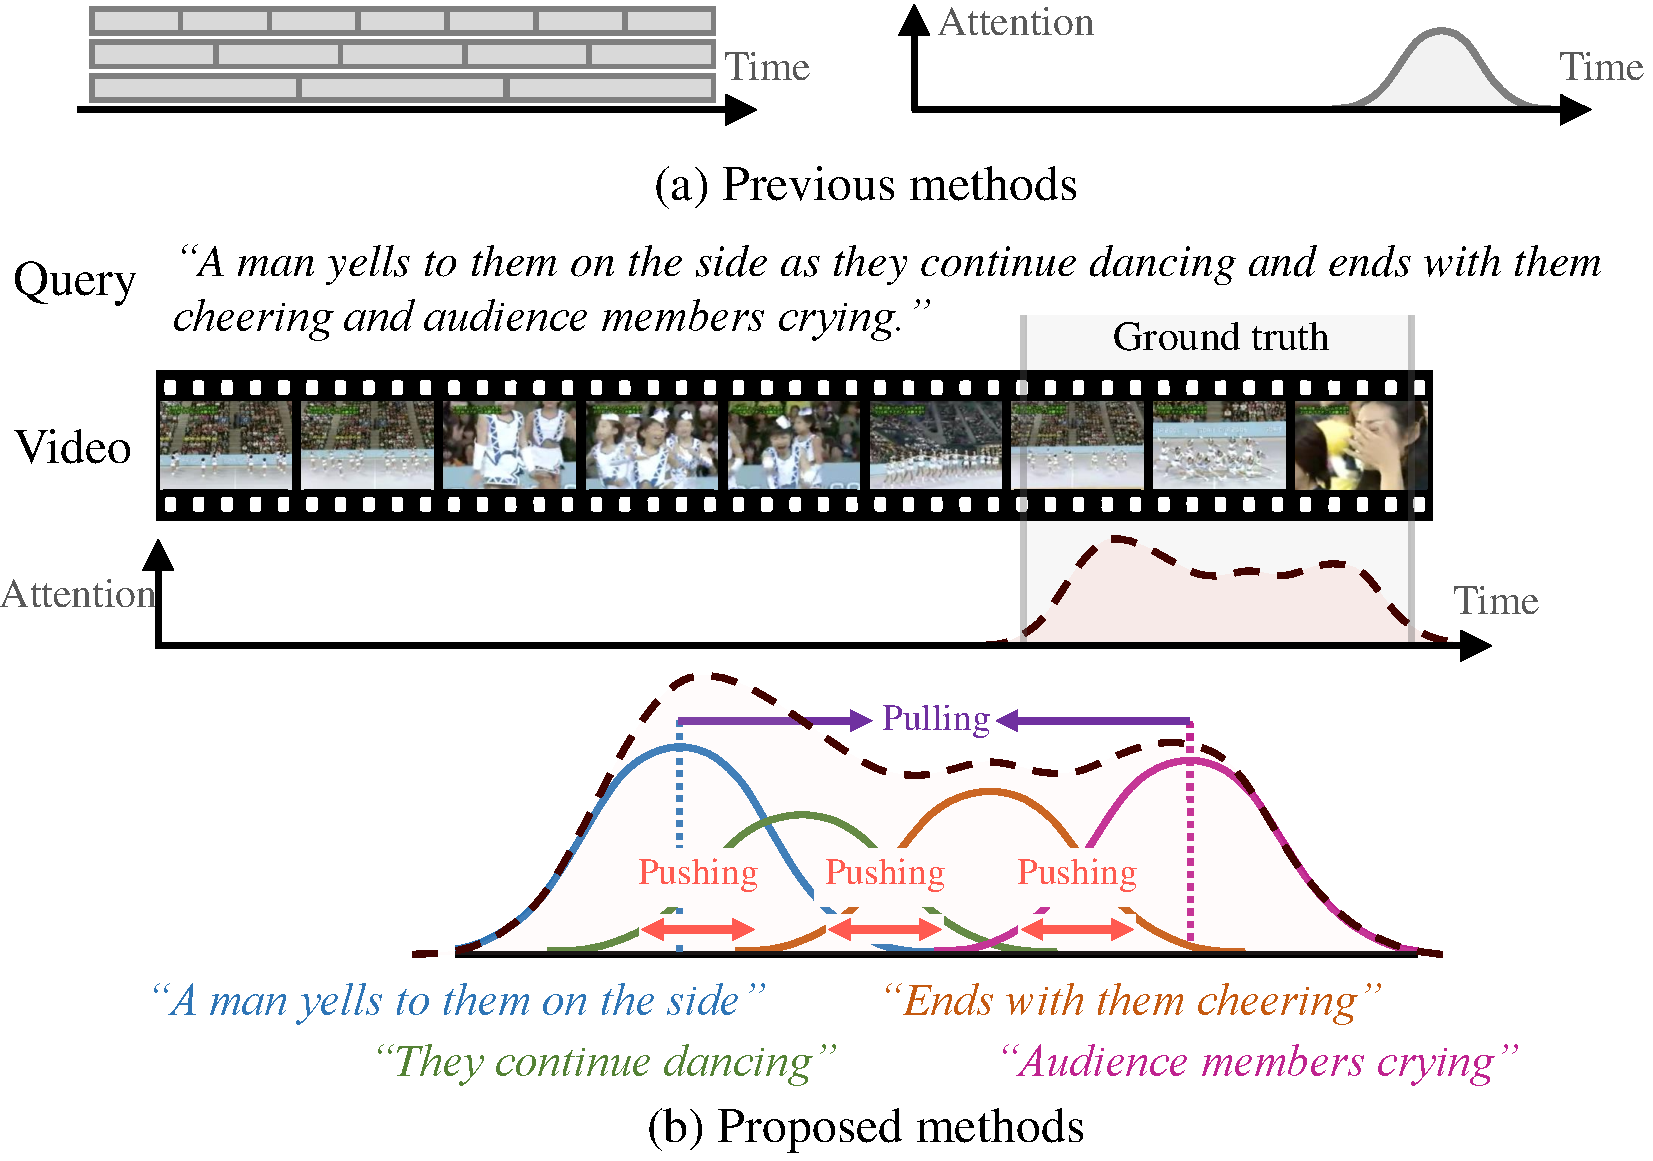
\includegraphics[width=\linewidth]{figures/0-concept-art.pdf}
  \caption{Weakly supervised temporal video grounding. (a) Previous methods use sliding windows (left) or a single Gaussian proposal (right), which has a predetermined shape. (b) The proposed method generates a Gaussian mixture proposal trained to be moderately coupled with a pull-push learning scheme to capture diverse query-relevant events.
  % Further, the proposed method leverages multiple learnable Gaussians for a negative proposal, instead of an existing rule-based one.
  }
\label{fig:concept-art}
\end{figure}

To overcome the limitation, a weakly supervised approach has been proposed to solve the temporal video grounding problem, where only video-sentence pairs are required for training. 
%% Weakly supervised video grounding methods %%%%%%%%%%%%%%%%%%%%%%%%%%%%%%
Some existing methods~\cite{huang2021cross, lin2020weakly, mithun2019weakly, tan2021logan, wang2021weakly, zhang2020counterfactual} use a sliding window strategy to generate proposals for a temporal location but use a lot of pre-defined proposals, which require heavy computation.
%and face difficulties in expressing diverse events described by the sentence query.
%% Gaussian-based methods %%%%%%%%%%%%%%%%%%%%%%%%%%%%%%
To reduce the required number of proposals, \cite{zheng2022cnm, zheng2022cpl} generate learnable Gaussian proposals. 
However, these single Gaussian proposals with a peak at its center lack the expression ability for diverse query-relevant events in a video.

To enhance the expression ability, we propose a Gaussian mixture proposal (GMP) that can depict arbitrary shapes by learning importance, centroid, and range of every Gaussian in the mixture.
% \cite{zong2018deep, lee2018simple}
Since our GMP is implemented over a temporal location, conventional feature-based learning for Gaussian mixture model~\cite{zong2018deep, lee2018simple} is not applicable to our approach.
In our special setting, our goal is to train the GMP to capture a temporal location semantically %relevant to a sentence query.
%We note that a temporal location 
relevant to a sentence query that includes diverse events coupled moderately. %coupled.
In \cref{fig:concept-art}, for instance, one sentence query includes two semantic events coupled by ``A man yells to them on the side" and ``They continue dancing".
%in the given sentence query have their own semantics but are moderately coupled to express one sentence query.

%% Proposed methods %%%%%%%%%%%%%%%%%%%%%%%%%%%%%%
To capture the %moderately 
coupled events in a query, we propose a Pull-Push Scheme (PPS) to learn a GMP whose Gaussians are moderately coupled.
Specifically, we first define a GMP with learnable parameters: importance, centroid, and range of every Gaussian in the mixture.
To learn the importance, we propose an importance weighting strategy that represents importance levels of each Gaussian mask for a query-relevant location.
To generate the GMP that represents a query-relevant location, our PPS is trained to reconstruct the sentence query from the proposal.
In our scheme, the Gaussians in one GMP should be located near a query-relevant temporal location, 
% but should not converge to an identical point to represent diverse events.
but should not be overlapped too much with others to represent diverse events.
To this end, our scheme leverages a pulling loss and a pushing loss, each of which plays an opposite role to the other to produce moderately coupled Gaussians.
The pulling loss lets the Gaussians stay close to each other by pulling the Gaussian centroids together.
% the two farthest masks together.
The pushing loss prevents the Gaussians from overlapping too much with the others by forcing the Gaussians to be less overlapped.

We verify that our scheme generates high-quality proposals that significantly improve recall rates on the Charades-STA~\cite{gao2017tall} and ActivityNet Captions~\cite{krishna2017dense} datasets.
We also demonstrate the effectiveness of each component in our scheme with extensive ablation studies.
%% Contributions %%%%%%%%%%%%%%%%%%%%%%%%%%%%%%
In summary, our contributions are as follows.
\begin{itemize}
\item We generate a Gaussian mixture proposal that represents a query-relevant temporal location by learning importance, centroid, and range of every Gaussian to enhance the expression ability of the proposal.
\item We propose a pull-push learning scheme that uses a pulling loss and a pushing loss, each of which plays an opposite role to the other to capture diverse events.
\item The proposed components are verified in-depth with extensive ablation studies and the overall scheme achieves state-of-the-art performance. 
\end{itemize}


\section{Related Work}
%% Related Works %%%%%%%%%%%%%%%%%%%%%%%%%%%%%%
\begin{figure*}[t!]
  \centering
  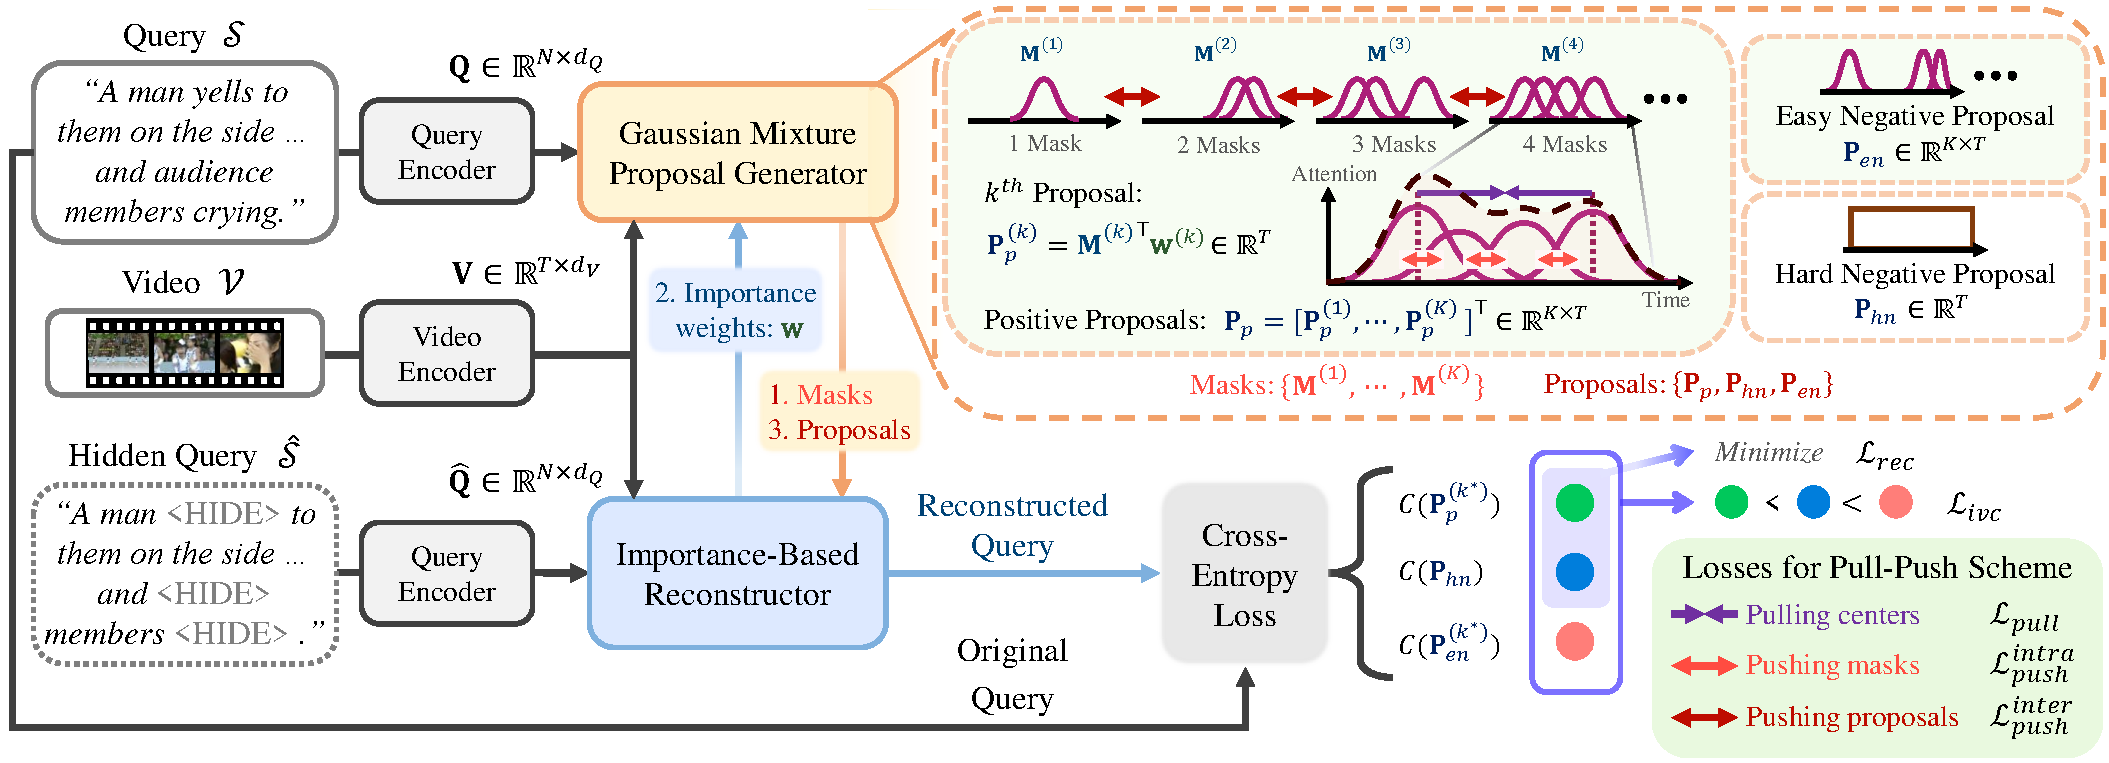
\includegraphics[width=\linewidth]{figures/1-framework.pdf}
  \caption{
  The overall scheme of the proposed method.
  % The proposal generator produces multiple Gaussian masks (positive, easy negative) and an entire video mask (hard negative) from the features representing both the video and sentence query.
  The Gaussian mixture proposal generator produces multiple Gaussian masks from the features representing both the video and sentence query.
  For the positive proposals, we define a Gaussian mixture proposal, where multiple Gaussian masks are combined via attentive pooling using the importance weights from the importance-based reconstructor.
  Further, to generate moderately coupled masks in the mixture proposal,
  we propose the pull-push learning scheme using $\mathcal{L}_{pull}$, $\mathcal{L}^{intra}_{push}$, and $\mathcal{L}^{inter}_{push}$.
  The importance-based reconstructor leverages the proposals to produce the reconstructed query from the hidden query. 
  % Our key contributions are highlighted with a green background.
  %For reconstruction, we minimize the cross-entropy losses of the positive proposals $\mathcal{L}_{rec}$.
  %To distinguish positive proposals from negative proposals, we perform contrastive learning with $\mathcal{L}_{ivc}$.
  }
\label{fig:framework}
\end{figure*}

% %% Fully supervised temporal video grounding %%%%%%%%%%%%%%%%%%%%%%%%%%%%%%
% \subsection{Fully supervised temporal video grounding}
% \label{sec:fully-supervised-temporal-video-grounding}
% %%%%%%%%%%%%%%%%%%%%%%%%%%%%%%%%%%%%%%%%%%%%%%%%%%%%%%%%
% % \textbf{Fully supervised temporal video grounding.}

% In fully supervised temporal video grounding, temporal locations of starting and ending times for every video-sentence pair are required during training.
% An early work~\cite{gao2017tall} makes sliding window-based proposals from a video and ranks the proposals according to the similarities between the proposal and the query.
% % Then, the proposal with the highest similarity is chosen as a predicted temporal location.
% % To make high-quality proposals, Xu \etal~\cite{xu2019multilevel} generate proposals guided by the query features to eliminate redundant proposals.
% % Also, Xiao \etal~\cite{xiao2021boundary} make high-quality proposals from an anchor-free model and use a visual-language fusion layer to model the multi-modal features.
% % To avoid heavy computations for generating proposals, proposal-free methods~\cite{ghosh2019excl, zeng2020dense} directly find temporal locations of starting and ending times without proposals.
% % Among the proposal-free methods, 
% The attention-based methods~\cite{yuan2019find, kim2021plrn} focus on specific video segments using a semantic phrase feature from the query.
% Similarly, multiple semantic phrases are leveraged for multi-level interaction between the query and video in \cite{mun2020local, kim2022swag}.
% However, the fully supervised methods require labor-intensive manual annotations of temporal locations which limit its scalability to real-world scenarios.
% Also, subjective annotations for temporal locations make trained models biased~\cite{yuan2021closer, zhou2021embracing}.
% Therefore, weakly supervised temporal video grounding has gained attention in recent years because it does not require temporal locations for video-sentence pairs.

%% Weakly supervised temporal video grounding %%%%%%%%%%%%%%%%%%%%%%%%%%%%%%
\subsection{Weakly Supervised Temporal Video Grounding}
\label{sec:weakly-supervised-temporal-video-grounding}
%%%%%%%%%%%%%%%%%%%%%%%%%%%%%%%%%%%%%%%%%%%%%%%%%%%%%%%%
% \textbf{Weakly supervised temporal video grounding.}

% In weakly supervised temporal video grounding, only video-sentence pairs are provided.

\paragraph{Sliding window-based methods}~\cite{huang2021cross, tan2021logan, mithun2019weakly, wang2021weakly, zhang2020counterfactual} generate proposals through the sliding window strategy and select the most probable proposal.
\cite{tan2021logan} proposes a multi-level co-attention model to learn visual-semantic representations.
\cite{huang2021cross} uses relations between sentences to understand cross-moment relations in videos.
However, sliding window-based methods make a lot of proposals with a predefined length and use Non-Maximum Suppression (NMS)~\cite{neubeck2006efficient} to reduce redundant proposals.
This process requires a large amount of computation. 
% and prior knowledge on the length distribution of temporal locations for each dataset.
The proposed method generates learnable Gaussian mixture proposals without using the sliding window.

\paragraph{Reconstruction-based methods}~\cite{lin2020weakly, zheng2022cnm, zheng2022cpl, song2020weakly, cao2023iterative} assume that well-generated proposals can reconstruct a sentence query from a randomly hidden sentence query.
Early works~\cite{lin2020weakly, song2020weakly} aggregate contextual information of video-sentence pairs to score proposals sampled at different scales.
However, these methods need to select one proposal from a large set of proposals, which requires heavy computation costs.
% song2020weakly is not sliding window-based
To solve this problem, other reconstruction-based methods~\cite{zheng2022cnm, zheng2022cpl} propose a learnable Gaussian proposal for a small set of proposals.
\cite{cao2023iterative} iteratively refines proposal confidence scores to prevent the grounding results from being biased.
Unlike the previous methods, our goal is to enhance the expression ability of proposals, hence we generate Gaussian mixture proposals which can effectively represent an arbitrary shape.
% and consider unmatched pairs of a sentence query and a video location inside the same video for contrastive learning.
% However, a Gaussian mask is a pre-determined shape with a high value on its center and lower values on its sides.
% Therefore, a single Gaussian mask is not suitable for expressing a temporal structure in a video because the temporal structure can be represented as an arbitrary shape with different importance according to the existence of semantic entities.


%% Gaussian Proposals in Video %%%%%%%%%%%%%%%%%%%%%%%
\subsection{Gaussian-based Approach}
\label{sec:gaussian-proposals-in-video}
%%%%%%%%%%%%%%%%%%%%%%%%%%%%%%%%%%%%%%%%%%%%%%%%%%%%%%%%

Gaussians have been studied in various tasks~\cite{zong2018deep, lee2018simple, piergiovanni2019temporal, long2019gaussian, zheng2022cnm, zheng2022cpl}.
For weakly-supervised temporal video grounding, \cite{zheng2022cnm, zheng2022cpl} propose learnable Gaussian proposals.
Specifically, \cite{zheng2022cnm} generates one Gaussian proposal for one temporal location, and \cite{zheng2022cpl} generates multiple Gaussian proposals and selects one proposal to predict a query-relevant temporal location.
% To depict an arbitrary shape of temporal structure, we make one Gaussian mixture proposal for one temporal location.
For action localization, 
\cite{long2019gaussian} uses multiple Gaussian proposals to localize multiple actions, where each single Gaussian proposal represents a temporal location of a specific action.
% Thus, the multiple Gaussian proposals do not work as a Gaussian mixture, which can not capture diverse events.

However, a single Gaussian is a pre-determined shape with a high value at its center, which is not suitable for expressing diverse query-relevant events.
To effectively represent the diverse events, we propose a Gaussian mixture proposal by learning importance, centroid, and range of every Gaussian in the mixture.
For action localization,
\cite{piergiovanni2019temporal} proposes a layer of Gaussian mixture that replaces a conventional convolutional layer to extract video features.
% Video features are applied to the Gaussian mixture layer to capture temporal information.
Also, there have been various tasks that train Gaussian mixture model in a feature space~\cite{zong2018deep, lee2018simple}.
Unlike these methods, we generate Gaussian mixture proposals that are directly implemented over a temporal location.
To represent a query-relevant temporal location that has diverse events, we propose a pull-push scheme to learn the moderately coupled Gaussian mixture.



\section{Proposed Method}
\section{Method}
In this work, we adapted the CaSSLe \cite{fini2022self} and Kaizen \cite{tang2023practical} continual learning frameworks to HAR. This section begins with an overview of these methods and then illustrates the modifications adopted to explore their application to HAR.

\subsection{CaSSLe}
The CaSSLe framework \cite{fini2022self} re-purposed the Siamese/Contrastive learning setup and loss functions for tackling catastrophic forgetting in representation learning. In particular, the framework consists of two main components: new task learning and knowledge distillation.
The \textbf{new task learning (feature extractor)} component follows the conventional Siamese/Contrastive learning setup, like that in BYOL~\cite{grill2020bootstrap} and MoCoV2+~\cite{chen2020improved, he2020momentum}, in which the input signal is transformed into two views using stochastic transformation functions, and the loss function forces the transformed view to have similar representations. The loss term for this is denoted by $\mathcal{L}^{\mathrm{CT}}_{\mathrm{FE}}$.
The \textbf{knowledge distillation (feature extractor)} component mirrors the new task learning component, where the same contrastive loss function is used again, but contrasting the representations retrieved by the feature extractor from the previous task and the current feature extractor instead. An additional predictor (a shallow neural network) is attached to the current feature extractor before contrastive learning. We denote this loss as $\mathcal{L}^{\mathrm{KD}}_{\mathrm{FE}}$.
The CaSSLe framework was shown to be an effective strategy for continual representation learning from a stream of unlabelled data, but it does not propose a specific strategy for training the downstream classifier continually.

\subsection{Kaizen}
The Kaizen framework \cite{tang2023practical} extends CaSSLe by proposing two additional components to handle classifier training, to ensure that a functional classifier is available at any step of the continual learning process.
The \textbf{new task learning (classifier)} component follows conventional supervised learning, in which the classifier is trained using categorical cross-entropy to learn the new classes ($\mathcal{L}^{\mathrm{CT}}_{\mathrm{C}}$).
The \textbf{knowledge distillation (classifier)} component leverages self-distillation to retain knowledge, in which the predictions from the classifier from the previous task are used as pseudo-labels to train the current classifier ($\mathcal{L}^{\mathrm{KD}}_{\mathrm{C}}$). This component does not rely on labelled data and can remain active when only unlabelled data is available.
A small part of the labelled data is retained and replayed, in a similar fashion to other exemplar-based continual learning methods \cite{rebuffi2017icarl, isele2018selective, rolnick2019experience, mittal2021essentials}. This was shown to be a critical component in maintaining classification performance in class-incremental settings \cite{de2021continual}.

\subsection{CSSL for HAR}
\label{subsec:balancing}
As both CaSSLe and Kaizen were proposed for visual representation learning in their original work, we made a few modifications to these frameworks to adapt to HAR.

\subsubsection{Transformation Functions}
Instead of using image transformation functions, we adopted three transformation functions from previous works \cite{har_transformations, multi_self_har, tang2020exploring, tang2021selfhar} that are tailored to sensor time-series: \emph{random 3D rotation}, \emph{random scaling} and \emph{time warping} (see Appx.~\ref{appx:trans}).

\subsubsection{Balancing Learning Objectives}

In addition to following the original formulation of Kaizen, in which the loss function is a sum of all the learning objectives mentioned above 
\[
 \mathcal{L_\mathrm{Kaizen}} =\mathcal{L}^{\mathrm{CT}}_{\mathrm{FE}} + \mathcal{L}^{\mathrm{KD}}_{\mathrm{FE}} + \mathcal{L}^{\mathrm{CT}}_{\mathrm{C}} + \mathcal{L}^{\mathrm{KD}}_{\mathrm{C}}
\]
we hypothesise that the relative importance of the knowledge distillation task compared to learning from new data in classification learning can have a direct impact on the performance of the classifier across time. Therefore, we introduce an importance coefficient $\lambda_{\mathrm{C}}$ to the loss function which allows us to change the weighting of the learning objectives:
\[
 \mathcal{L_\mathrm{Kaizen(adaptive)}} =(\mathcal{L}^{\mathrm{CT}}_{\mathrm{FE}} + \mathcal{L}^{\mathrm{KD}}_{\mathrm{FE}}) + (\mathcal{L}^{\mathrm{CT}}_{\mathrm{C}} + \lambda_{\mathrm{C}} \mathcal{L}^{\mathrm{KD}}_{\mathrm{C}})
\]
The effects of this importance coefficient are explored in our evaluation.


\section{Experiments}
%% Experiments %%%%%%%%%%%%%%%%%%%%%%%%%%%%%% 

% %% Datasets %%%%%%%%%%%%%%%%%%%%%%%%%%%%%%
% \subsection{Datasets}
% \label{sec:datasets}
% %%%%%%%%%%%%%%%%%%%%%%%%%%%%%%%%%%%%%%%%%%%%%%%%%%%%%%%%%%%%


%% Experimental setup %%%%%%%%%%%%%%%%%%%%%%%%%%%%%%
\subsection{Experimental Setup}
\label{sec:experimental-setup}
%%%%%%%%%%%%%%%%%%%%%%%%%%%%%%%%%%%%%%%%%%%%%%%%%%%%%%%%%%%%

%% Evaluation Metrics %%%%%%%%%%%%%%%%%%%%%%%%%%%%%%
% \subsection{Evaluation metrics}
% \label{sec:evaluation-metrics}
%%%%%%%%%%%%%%%%%%%%%%%%%%%%%%%%%%%%%%%%%%%%%%%%%%%%%%%%%%%%
\paragraph{Evaluation metrics.} Following the evaluation metrics in \cite{gao2017tall}, we adopt two metrics (`R@$n$,IoU=$m$' and `R@$n$,mIoU').
`R@$n$,IoU=$m$' denotes the percentage of at least one of the top-$n$ predicted temporal locations having a temporal Intersection over Union (IoU) with a ground truth larger than $m$.
`R@$n$,mIoU' denotes the average of the highest IoUs among the $n$ predicted temporal locations.
% On the ActivityNet-Captions dataset, we set the predefined $n$ to 1 or 5 and $m$ to 0.1, 0.3 or 0.5.
% On the Charades-STA dataset, we set the predefined $n$ to 1 or 5 and $m$ to 0.3, 0.5 or 0.7.

\begin{table}[t!]
  \centering
  \resizebox{\columnwidth}{!}{
  \begin{tabular}{l ccc ccc}
    \toprule
    \multirow{2}{*}{Method} & \multicolumn{3}{c}{R@1,IoU=} & \multicolumn{3}{c}{R@5,IoU=} \\ 
     & 0.1 & 0.3 & 0.5 & 0.1 & 0.3 & 0.5\\
    \midrule
    Random & 38.23 & 18.64 & 7.63 & 75.74 & 52.78 & 29.49 \\
    WS-DEC & 62.71 & 41.98 & 23.34 & - & - & - \\
    MARN & - & 47.01 & 29.95 & - & 72.02 & 57.49 \\
    VCA & 67.96 & 50.45 & 31.00 & 92.14 & 71.79 & 53.83 \\
    EC-SL & 68.48 & 44.29 & 24.16 & - & - & - \\
    % BAR~\cite{wu2020reinforcement} & - & 49.03 & 30.73 & - & - & - \\
    SCN & 71.48 & 47.23 & 29.22 & 90.88 & 71.56 & 55.69 \\
    RTBPN & 73.73 & 49.77 & 29.63 & 93.89 & 79.89 & 60.56 \\
    % CTF~\cite{chen2020look} & 74.20 & 44.30 & 23.60 & - & - & - \\
    % WSLLN~\cite{gao2019wslln} & 75.40 & 42.80 & 22.70 & - & - & - \\
    LCNet & 78.58 & 48.49 & 26.33 & 93.95 & 82.51 & 62.66 \\
    CCL & - & 50.12 & 31.07 & - & 77.36 & 61.29 \\
    WSTAN & 79.78 & 52.45 & 30.01 & 93.15 & 79.38 & 63.42 \\
    FSAN & 78.45 & 55.11 & 29.43 & 92.59 & 76.79 & 63.32 \\
    CWSTG & 71.86 & 46.62 & 29.52 & 93.75 & 80.92 & 66.61 \\
    % MSCL~\cite{mo2022multi} & 75.61 & 55.05 & \textbf{38.23} & 95.26 & 82.72 & 68.05\\
    CPL & \underbar{82.55} & 55.73 & 31.37 & 87.24 & 63.05 & 43.13 \\
    \midrule
    CRM$^*$ & 81.61 & 55.26 & 32.19 & - & - & - \\
    CNM$^*$ & 78.13 & 55.68 & \underbar{33.33} & - & - & - \\
    IRON$^*$ & \textbf{84.42} & \underbar{58.95} & \textbf{36.27} & \textbf{96.74} & \textbf{85.60} & \underbar{68.52} \\
    \midrule
    PPS & 81.84 & \textbf{59.29} & 31.25 & \underbar{95.28} & \underbar{85.54} & \textbf{71.32} \\
    \bottomrule
  \end{tabular}}
  \caption{Performance comparisons on the ActivityNet Captions. The best results and second best results are represented as bold and underlined numbers, respectively. The methods using additional annotations or large-scale pre-trained models are marked with $^*$.} 
  % \\ \small{$^*$: using additional annotations or large-scale pre-trained model.}
  \label{tab:comparisons-activitynet}
\end{table}





% \begin{table}[t!]
%   \centering
%   \resizebox{\columnwidth}{!}{
%   \begin{tabular}{l ccc ccc}
%     \toprule
%     \multirow{2}{*}{Method} & \multicolumn{3}{c}{R@1} & \multicolumn{3}{c}{R@5} \\ 
%      & IoU=0.1 & IoU=0.3 & IoU=0.5 & IoU=0.1 & IoU=0.3 & IoU=0.5\\
%     \midrule
%     Random & 38.23 & 18.64 & 7.63 & 75.74 & 52.78 & 29.49 \\
%     WS-DEC & 62.71 & 41.98 & 23.34 & - & - & - \\
%     MARN & - & 47.01 & 29.95 & - & 72.02 & 57.49 \\
%     VCA & 67.96 & 50.45 & 31.00 & 92.14 & 71.79 & 53.83 \\
%     EC-SL & 68.48 & 44.29 & 24.16 & - & - & - \\
%     % BAR~\cite{wu2020reinforcement} & - & 49.03 & 30.73 & - & - & - \\
%     SCN & 71.48 & 47.23 & 29.22 & 90.88 & 71.56 & 55.69 \\
%     RTBPN & 73.73 & 49.77 & 29.63 & 93.89 & 79.89 & 60.56 \\
%     % CTF~\cite{chen2020look} & 74.20 & 44.30 & 23.60 & - & - & - \\
%     % WSLLN~\cite{gao2019wslln} & 75.40 & 42.80 & 22.70 & - & - & - \\
%     LCNet & 78.58 & 48.49 & 26.33 & 93.95 & 82.51 & 62.66 \\
%     CCL & - & 50.12 & 31.07 & - & 77.36 & 61.29 \\
%     WSTAN & 79.78 & 52.45 & 30.01 & 93.15 & 79.38 & 63.42 \\
%     FSAN & 78.45 & 55.11 & 29.43 & 92.59 & 76.79 & 63.32 \\
%     CWSTG & 71.86 & 46.62 & 29.52 & 93.75 & 80.92 & 66.61 \\
%     % MSCL~\cite{mo2022multi} & 75.61 & 55.05 & \textbf{38.23} & 95.26 & 82.72 & 68.05\\
%     CPL & \underbar{82.55} & 55.73 & 31.37 & 87.24 & 63.05 & 43.13 \\
%     \midrule
%     CRM$^*$ & 81.61 & 55.26 & 32.19 & - & - & - \\
%     CNM$^*$ & 78.13 & 55.68 & \underbar{33.33} & - & - & - \\
%     IRON$^*$ & \textbf{84.42} & \underbar{58.95} & \textbf{36.27} & \textbf{96.74} & \textbf{85.60} & \underbar{68.52} \\
%     \midrule
%     PPS & 81.84 & \textbf{59.29} & 31.25 & \underbar{95.28} & \underbar{85.54} & \textbf{71.32} \\
%     \bottomrule
%   \end{tabular}}
%   \caption{Performance comparisons on the ActivityNet Captions. The best results and second best results are represented as bold and underlined numbers, respectively. The methods using additional annotations or large-scale pre-trained models are marked with $^*$.} 
%   % \\ \small{$^*$: using additional annotations or large-scale pre-trained model.}
%   \label{tab:comparisons-activitynet}
% \end{table}




%% ActivityNet Captions Dataset %%%%%%%%%%%%%%%%%%%%%%%%%%%%%%
\paragraph{The ActivityNet Captions dataset}~\cite{krishna2017dense}
contains 37,417, 17,505, and 17,031 video-sentence pairs for training, validating $val_1$, and $val_2$, respectively.
Since a testing set is not publicly available, $val_2$ is used for testing.
Video segment features are extracted via C3D~\cite{tran2015learning}.
Vocabulary sizes are 8,000.
For proposals, $K$, $E_{en}$, and $\sigma$ are set to $5$, $2$, and $4$.
For losses, $\alpha_1$, $\alpha_2$, $\alpha_3$, and $\alpha_4$ are set to $1$, $0.2$, $0.01$, and $0.1$.

%% Charades-STA Dataset %%%%%%%%%%%%%%%%%%%%%%%%%%%%%%
\paragraph{The Charades-STA dataset}~\cite{gao2017tall}
contains 16,128 video-sentence pairs from 6,672 videos, which are divided into 12,408 for training and 3,720 for testing.
Video segment features are extracted via I3D~\cite{carreira2017quo}.
Vocabulary sizes are 1,111.
For proposals, $K$, $E_{en}$, and $\sigma$ are set to $7$, $3$, and $9$.
For losses, $\alpha_1$, $\alpha_2$, $\alpha_3$, and $\alpha_4$ are set to $3$, $5$, $0.001$, and $1$.

\paragraph{Implementation details.} We set the maximum number of video segments to 200, and the maximum length of the sentence query to 20.
For the transformers, we use transformers with three-layer and four attention heads.
The dimension of the features ($d_V$, $d_Q$, $d_G$, $d_R$) is set to 256.
We use the equivalent MC Transformer for every reconstruction process.
For the hidden sentence query, we randomly hide a third ($1/3$) of the words.
For training, the Adam optimizer~\cite{kingma2014adam} is used.
We set the learning rate to 0.0004, mini-batch size to 32, and hyper-parameters as $\lambda_1=\lambda_2=0.15$, $\beta_1=0.1$, and $\beta_2=0.15$.
In the $k^{th}$ positive proposal, we set the number of Gaussian masks $E_p$ to $k$ for reflecting a varying number of masks in each proposal, as shown in the top right of \cref{fig:framework}.
% More implementation details are described in Supplementary material.

\begin{table*}[t!]
  \centering
  \resizebox{0.95\linewidth}{!}{
  \begin{tabular}{cc c cccc}
    \toprule
    \multirow{2}{*}{Component} & \multirow{2}{*}{Strategy} & Loss & \multicolumn{2}{c}{R@1} & \multicolumn{2}{c}{R@5} \\ 
     &  & $\mathcal{L}_{pull}$ \& $\mathcal{L}^{intra}_{push}$ & IoU=0.3 & mIoU & IoU=0.3 & mIoU \\
    \midrule
    \multirow{2}{*}{Proposal type} 
     & Single Gaussian & \xmark & 47.49 & 33.33 & 78.23 & 54.85 \\
     & Gaussian mixture & \cmark & \textbf{59.29} & \textbf{37.59} & \textbf{85.54} & \textbf{58.78} \\
    \midrule
    \multirow{3}{*}{Gaussian generation} 
     & Learning one center \& multiple widths & \xmark & 46.63 & 31.54 & 83.65 & \textbf{59.49} \\
     & Learning multiple centers \& widths & \cmark & 47.82 & 32.08 & 84.09 & 56.35 \\ 
     & Learning multiple centers \& one width  & \cmark & \textbf{59.29} & \textbf{37.59} & \textbf{85.54} & 58.78 \\
     \midrule
     \multirow{3}{*}{Importance weighting} & No importance & \cmark & 52.55 & 34.56 & 79.67 & 58.41 \\
     & Importance from the generator & \cmark & 48.55 & 32.36 & 78.96 & 56.87 \\ 
     & Importance from the reconstructor & \cmark & \textbf{59.29} & \textbf{37.59} & \textbf{85.54} & \textbf{58.78} \\ 
    \bottomrule
  \end{tabular}
  }
  \caption{Ablation studies of Gaussian mixture proposals on the ActivityNet Captions dataset.}

  \label{tab:ablation-positive-proposals}
\end{table*}

 
\begin{table}[t!]
  \centering
  \resizebox{\columnwidth}{!}{
  \begin{tabular}{l ccc ccc}
    \toprule
    \multirow{2}{*}{Method} & \multicolumn{3}{c}{R@1,IoU=} & \multicolumn{3}{c}{R@5,IoU=} \\ 
     & 0.3 & 0.5 & 0.7 & 0.3 & 0.5 & 0.7\\
    \midrule
    Random & 20.12 & 8.61 & 3.39 & 68.42 & 37.57 & 14.98 \\
    TGA & 32.14 & 19.94 & 8.84 & 86.58 & 65.52 & 33.51 \\
    % CTF~\cite{chen2020look} & 39.80 & 27.30 & 12.90 & -  & - & - \\
    SCN & 42.96 & 23.58 & 9.97 & 95.56 & 71.80 & 38.87 \\
    WSTAN & 43.39 & 29.35 & 12.28 & 93.04 & 76.13 & 41.53 \\
    % BAR~\cite{wu2020reinforcement} & 44.97 & 27.04 & 12.23 & -  & - & - \\
    VLANet & 45.24 & 31.83 & 14.17 & 95.70 & 82.85 & 33.09 \\
    MARN & 48.55 & 31.94 & 14.81 & 90.70 & 70.00 & 37.40 \\
    % WSRA~\cite{fang2020weak} & 50.13 & 31.20 & 11.01 & 86.75 & 70.50 & 39.02 \\
    CCL & - & 33.21 & 15.68 & - & 73.50 & 41.87 \\
    RTBPN & 60.04 & 32.36 & 13.24 & 97.48 & 71.85 & 41.18 \\
    LoGAN & 51.67 & 34.68 & 14.54 & 92.74 & 74.30 & 39.11 \\
    VCA & 58.58 & 38.13 & 19.57 & 98.08 & 78.75 & 37.75 \\
    LCNet & 59.60 & 39.19 & 18.87 & 94.78 & 80.56 & 45.24 \\
    CWSTG & 43.31 & 31.02 & 16.53 & 95.54 & 77.53 & 41.91 \\
    % MSCL~\cite{mo2022multi} & 58.92 & 43.15 & 23.49 & 98.02 & 81.23 & 48.45 \\
    CPL & 66.40 & 49.24 &
    22.39 & 96.99 & 84.71 & 52.37 \\
    \midrule
    CRM$^*$ & 53.66 & 34.76 & 16.37 & -  & - & - \\
    CNM$^*$ & 60.39 & 35.43 & 15.45 & -  & - & - \\
    IRON$^*$ & \textbf{70.71} & \textbf{51.84} & \underbar{25.01} & \underbar{98.96} & \textbf{86.80} & \textbf{54.99} \\
    \midrule
    PPS & \underbar{69.06} & \underbar{51.49} & \textbf{26.16} & \textbf{99.18} & \underbar{86.23} & \underbar{53.01} \\
    \bottomrule
  \end{tabular}}
  \caption{Performance comparisons on the Charades-STA.
  The best results and second best results are represented as bold and underlined numbers, respectively. The methods using additional annotations or large-scale pre-trained models are marked with $^*$.} 
  % \\ \small{$^*$: using additional annotations or large-scale pre-trained model.}
  \label{tab:comparisons-charades}
\end{table}




% \begin{figure}[t!]
%   \centering
%     \begin{subfigure}[b]{\linewidth}
%          \centering
%          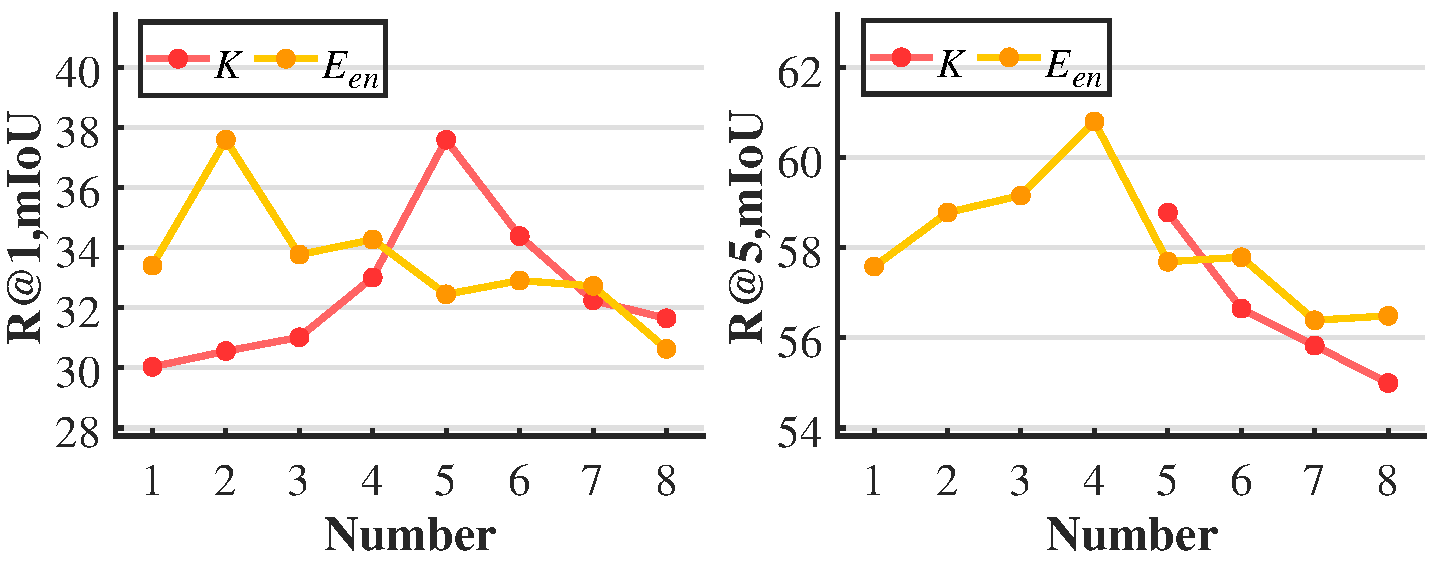
\includegraphics[width=\linewidth]{figures/3-ablation-graph-props.pdf}
%          \caption{}
%          \label{fig:ablation-graph-props}
%     \end{subfigure}
%     \vfill
%     \begin{subfigure}[b]{\linewidth}
%          \centering
%          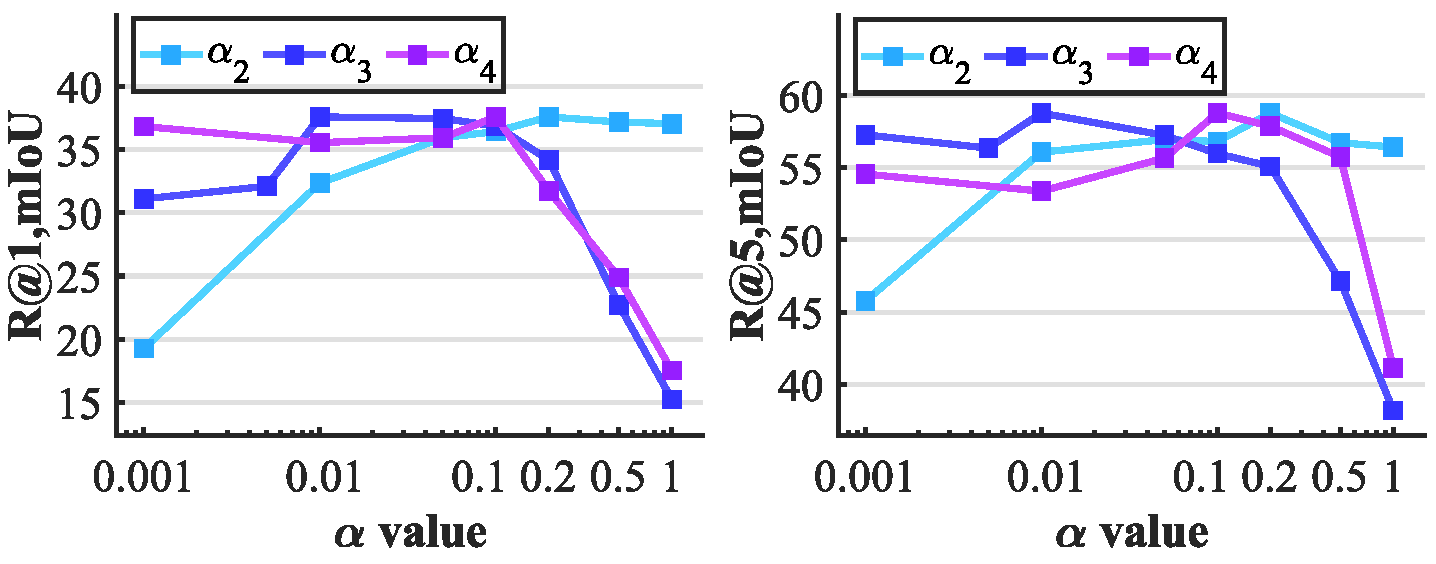
\includegraphics[width=\linewidth]{figures/3-ablation-graph-alpha.pdf}
%          \caption{}
%          \label{fig:ablation-graph-alpha}
%     \end{subfigure}
%     \caption{Ablation studies by varying (a) the number of proposals $K$ and the number of negative masks $E_{en}$ for each easy negative proposal and (b) $\alpha$ values for the pull-push learning scheme on the ActivityNet Captions dataset.
%     % $\alpha$, $\alpha_3$, and $\alpha_4$ for balancing losses
%     }
% \label{fig:ablation-graph}
% \end{figure}

%% Comparison with State-of-the-Arts %%%%%%%%%%%%%%%%%%%%%%%%%%%%%%
\subsection{Comparison with State-of-the-Art Methods}
\label{sec:comparison-with-state-of-the-art-methods}
%%%%%%%%%%%%%%%%%%%%%%%%%%%%%%%%%%%%%%%%%%%%%%%%%%%%%%%%%%%%
To verify the effectiveness of the proposed method, we compare our PPS with previous weakly supervised temporal video grounding methods:
WS-DEC~\cite{duan2018weakly},
TGA~\cite{mithun2019weakly},
SCN~\cite{lin2020weakly},
WSTAN~\cite{wang2021weakly},
VLANet~\cite{ma2020vlanet},
MARN~\cite{song2020weakly},
CCL~\cite{zhang2020counterfactual},
RTBPN~\cite{zhang2020regularized},
EC-SL~\cite{chen2021towards},
LoGAN~\cite{tan2021logan},
VCA~\cite{wang2021visual},
LCNet~\cite{yang2021local},
FSAN~\cite{wang2022fine},
CWSTG~\cite{Chen_Luo_Zhang_Ma_2022},
CPL~\cite{zheng2022cpl},
CRM~\cite{huang2021cross},
CNM~\cite{zheng2022cnm}, and
IRON~\cite{cao2023iterative}.

In \cref{tab:comparisons-activitynet} for the ActivityNet Captions dataset, our PPS outperforms CPL~\cite{zheng2022cpl} by $3.56\%$, $22.49\%$, and $28.19\%$ at R@1,IoU=0.3, R@5,IoU=0.3, and R@5,IoU=0.5, respectively.
It is worth noting that PPS outperforms the previous learnable mask-based method, CPL, by significant margins at R@5, which means that the generated proposals of PPS promise a higher level of quality.
In \cref{tab:comparisons-charades} for the Charades-STA dataset, our PPS surpasses CPL~\cite{zheng2022cpl} by $3.77\%$ and $2.19\%$ at R@1,IoU=0.7 and R@5,IoU=0.3, respectively.
The methods marked with $^*$ make unfair comparisons with the previous methods.
CRM~\cite{huang2021cross} uses additional paragraph description annotations. CNM~\cite{zheng2022cnm} uses CLIP large-scale pre-trained features~\cite{radford2021learning} and IRON~\cite{cao2023iterative} uses OATrans~\cite{wang2022object} and DistilBERT~\cite{sanh2019distilbert} large-scale pre-trained features.
Although our PPS uses 3D ConvNet and Glove features for fair comparisons with previous methods, PPS shows competitive or higher performance with the methods marked with $^*$.
% To study the impact of large-scale pre-trained features, we conduct the experiment using CLIP features in Supplementary material.

\begin{figure}[t!]
  \centering
  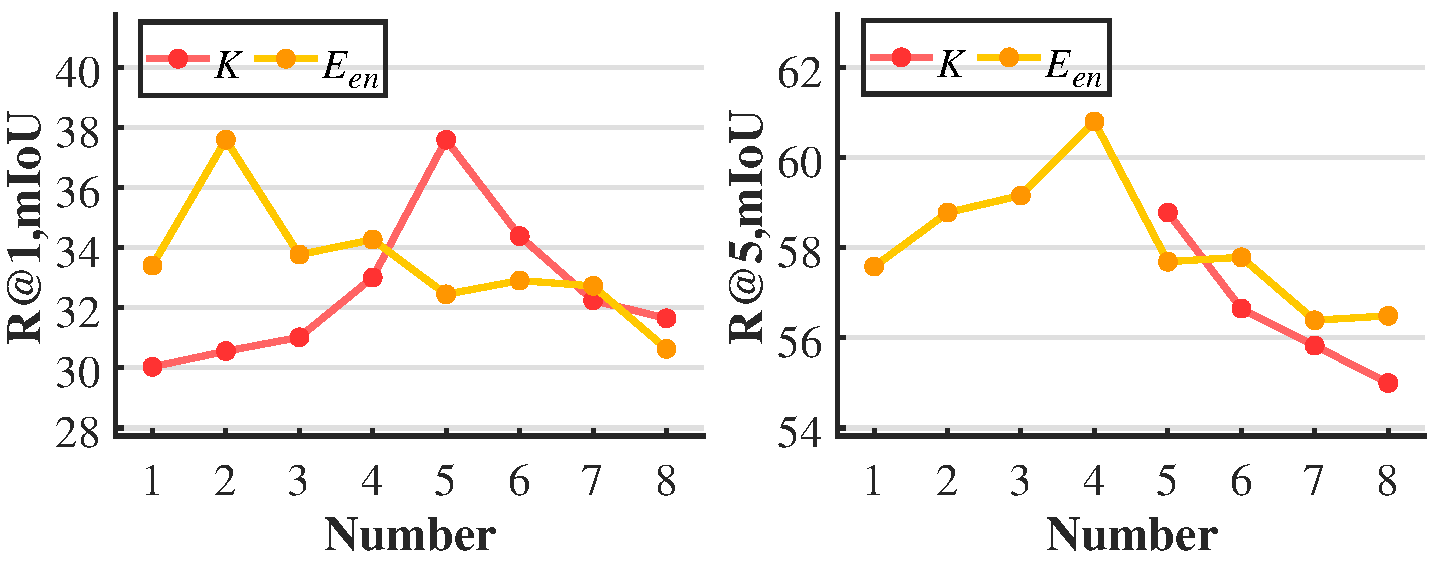
\includegraphics[width=\linewidth]{figures/3-ablation-graph-props.pdf}
    \caption{Ablation studies by varying the number of positive and negative proposals $K$ and the number of Gaussian masks of an easy negative proposal $E_{en}$.
    }
    \label{fig:ablation-graph-props}
\end{figure}

%% Ablation Study %%%%%%%%%%%%%%%%%%%%%%%%%%%%%%
\subsection{Ablation Study}
\label{sec:ablation-study}
%%%%%%%%%%%%%%%%%%%%%%%%%%%%%%%%%%%%%%%%%%%%%%%%%%%%%%%%%%%%
For a more in-depth understanding of the proposed method, we perform ablation studies on our components.
% More details of the variants used in the ablation studies are explained in Supplementary material.

\paragraph{Analysis on the Gaussian mixture proposal.}
As shown in \cref{tab:ablation-positive-proposals}, we study the impact of the different strategies to generate Gaussian mixture proposals for positive proposals.
The results are summarized as follows:
First, the Gaussian mixture proposals are more effective than the single Gaussian proposal, which means that the mixture proposal can better represent a query-relevant temporal location.
Second, learning multiple centers and one width for one mixture proposal performs best.
We conjecture that learning multiple widths makes it complicated to learn proposals, which reduces performance.
Third, importance weighting from the reconstructor yields the best result by representing the importance of each mask for query reconstruction.
On the other hand, importance weighting from the generator is less effective, because it is hard to reflect reconstruction-aware information.
\cref{fig:ablation-graph-props} shows the impact of the number of proposals $K$.
The performance increases until the number is $5$ at R@1,mIoU.
We observe that defining too many proposals makes the proposals redundant and have short lengths due to the impact of the inter-pushing loss $\mathcal{L}^{inter}_{push}$.


\paragraph{Impact on a varying number of masks.}
For positive proposals, we form $\mathbf{P}_{p}^{(k)}$ by a Gaussian mixture of $E_p=k$ Gaussian masks to reflect a varying number of Gaussian masks in each positive proposal.
To verify the effectiveness of the varying number of Gaussian masks, we compare the performance of fixing the number of Gaussian masks for every positive proposal in \cref{tab:ablation-positive-proposals-fixing}.
The results show that using a varying number of Gaussian masks for each positive proposal performs better than using a fixed Gaussian number of Gaussian masks.
We find that combinations of different numbers of Gaussian masks can represent a diverse number of query-relevant events.

\begin{table}[t!]
  \centering
          \begin{subtable}[t]{.47\linewidth}
            \centering
              \resizebox{\columnwidth}{!}{
              \begin{tabular}{c cc}
                \toprule
                \multirow{2}{*}{\# masks} & R@1 & R@5 \\ 
                 & mIoU & mIoU \\
                \midrule
                Fix to 1 & 33.33 & 54.85 \\ 
                Fix to 3 & 35.91 & 56.27 \\ 
                Fix to 5 & 36.58 & 54.36 \\ 
                Fix to 7 & 36.25 & 49.48 \\ 
                \midrule
                Vary & \textbf{37.59} & \textbf{58.78} \\ 
                \bottomrule
          \end{tabular}}
        \caption{The number of masks for a positive proposal.}
          \label{tab:ablation-positive-proposals-fixing}
            \end{subtable}%
        \hspace{0.2cm}
        \begin{subtable}[t]{.47\linewidth}
                  \centering
                      \resizebox{\columnwidth}{!}{
                      \begin{tabular}{c cc}
                        \toprule
                        Pulling & R@1 & R@5 \\ 
                        strategy & mIoU & mIoU \\
                        \midrule
                        All & 35.41 & 56.87 \\ 
                        To mid & 35.83 & \textbf{58.92} \\ 
                        Distant & \textbf{37.59} & 58.78 \\ 
                        \bottomrule
                \end{tabular}}
                \caption{Strategies for the pulling loss}
              \label{tab:ablation-pulling-loss}
        \end{subtable}%
        \caption{Ablation studies on the ActivityNet Captions dataset.}
    % \hspace{0.5cm}
  %   \begin{subtable}[t]{.335\linewidth}
  %       \centering
  %             \caption{Ablation studies of hard \& easy negative proposals.}
  %             \resizebox{\columnwidth}{!}{
  %             \begin{tabular}{cc cc}
  %               \toprule
  %               \multirow{2}{*}{Negative proposal} & \multirow{2}{*}{$\mathcal{L}_{ivc}$} & R@1 & R@5 \\ 
  %                &  & mIoU & mIoU \\
  %               \midrule
  %               None & \xmark & 31.44 & 53.08 \\ 
  %               Only hard & \cmark & 32.49 & 56.23 \\ 
  %               Only easy & \cmark & 30.75 & 57.21 \\ 
  %               Both hard \& easy & \cmark & \textbf{37.59} & \textbf{58.78} \\ 
  %               \bottomrule
  %         \end{tabular}}
  %         \label{tab:ablation-negative-proposal-loss}
          
  % \end{subtable}
  \label{tab:ablation-others}
\end{table}



% \begin{table*}[t!]
%   \centering
%   \caption{Ablation studies on different strategies of PPS on the ActivityNet Captions dataset.}
%           \begin{subtable}[t]{.275\linewidth}
%             \centering
%               \caption{Performance comparisons by fixing the number of masks.}
%               \resizebox{\columnwidth}{!}{
%               \begin{tabular}{c cc}
%                 \toprule
%                 \multirow{2}{*}{Positive proposal} & R@1 & R@5 \\ 
%                  & mIoU & mIoU \\
%                 \midrule
%                 Varying num & \textbf{37.59} & \textbf{58.78} \\ \midrule
%                 Fixing to 1 & 33.33 & 54.85 \\ 
%                 Fixing to 3 & 35.91 & 56.27 \\ 
%                 Fixing to 5 & 36.58 & 54.36 \\ 
%                 Fixing to 7 & 36.25 & 49.48 \\ 
%                 \bottomrule
%           \end{tabular}}
%           \label{tab:ablation-positive-proposals-fixing}
%             \end{subtable}%
%         \hspace{0.5cm}
%         \begin{subtable}[t]{.31\linewidth}
%                   \centering
%                       \caption{Performance comparisons by varying strategies for the pulling loss $\mathcal{L}_{pull}$.}
%                       \resizebox{\columnwidth}{!}{
%                       \begin{tabular}{c cc}
%                         \toprule
%                         \multirow{2}{*}{$\mathcal{L}_{pull}$ strategy} & R@1 & R@5 \\ 
%                         & mIoU & mIoU \\
%                         \midrule
%                         Pulling all masks & 35.41 & 56.87 \\ 
%                         Pulling to the mid & 35.83 & \textbf{58.92} \\ 
%                         Pulling distant masks & \textbf{37.59} & 58.78 \\ 
%                         \bottomrule
%                 \end{tabular}}
%               \label{tab:ablation-pulling-loss}
%         \end{subtable}%
%     \hspace{0.5cm}
%   %   \begin{subtable}[t]{.335\linewidth}
%   %       \centering
%   %             \caption{Ablation studies of hard \& easy negative proposals.}
%   %             \resizebox{\columnwidth}{!}{
%   %             \begin{tabular}{cc cc}
%   %               \toprule
%   %               \multirow{2}{*}{Negative proposal} & \multirow{2}{*}{$\mathcal{L}_{ivc}$} & R@1 & R@5 \\ 
%   %                &  & mIoU & mIoU \\
%   %               \midrule
%   %               None & \xmark & 31.44 & 53.08 \\ 
%   %               Only hard & \cmark & 32.49 & 56.23 \\ 
%   %               Only easy & \cmark & 30.75 & 57.21 \\ 
%   %               Both hard \& easy & \cmark & \textbf{37.59} & \textbf{58.78} \\ 
%   %               \bottomrule
%   %         \end{tabular}}
%   %         \label{tab:ablation-negative-proposal-loss}
          
%   % \end{subtable}
%   \label{tab:ablation-others}
% \end{table*}



  
\begin{table}[t!]
  \centering
  \resizebox{\columnwidth}{!}{
  \begin{tabular}{ccc cccc}
    \toprule
    \multicolumn{3}{c}{Loss} & \multicolumn{2}{c}{R@1,IoU=} & \multicolumn{2}{c}{R@5,IoU=} \\ 
    $\mathcal{L}_{pull}$ & $\mathcal{L}^{intra}_{push}$ & $\mathcal{L}^{inter}_{push}$ & 0.3 & mIoU & 0.3 & mIoU \\
    \midrule
    \xmark & \xmark & \xmark & 45.23 & 30.98 & 67.86 & 47.75 \\
    \cmark & \xmark & \xmark & 55.03 & 36.79 & 72.49 & 51.14 \\
    \xmark & \cmark & \xmark & 45.69 & 29.83 & 71.51 & 49.69 \\
    \xmark & \xmark & \cmark & 23.50 & 15.96 & 72.30 & 44.46 \\
    \xmark & \cmark & \cmark & 23.47 & 16.38 & 66.15 & 38.20 \\
    \cmark & \xmark & \cmark & 41.51 & 30.23 & 85.18 & \textbf{60.44} \\
    \cmark & \cmark & \xmark & 49.98 & 32.46 & 80.54 & 55.26 \\ 
    \cmark & \cmark & \cmark & \textbf{59.29} & \textbf{37.59} & \textbf{85.54} & 58.78 \\ 
    \bottomrule
  \end{tabular}}
  \caption{Ablation studies of different losses for the pull-push learning scheme on the ActivityNet Captions dataset.}
  \label{tab:ablation-loss}
\end{table}



\paragraph{Effect of the pull-push learning scheme.}
In \cref{tab:ablation-loss}, we verify the effectiveness of our pull-push learning scheme.
Among combinations of three losses ($\mathcal{L}_{pull}$, $\mathcal{L}^{intra}_{push}$, $\mathcal{L}^{inter}_{push}$), adopting all three losses yields the best performance.
We conjecture that our pull-push learning scheme helps Gaussian masks to capture diverse events for better representing a temporal location.
It is notable that adopting only the pulling loss can yield competitive or higher results to the state-of-the-art methods in \cref{tab:comparisons-activitynet}.
If the pulling loss $\mathcal{L}_{pull}$ is excluded, the performance decreases significantly.
We observe that Gaussian masks for one Gaussian mixture proposal are spread sparsely throughout the entire video without $\mathcal{L}_{pull}$, which can not represent one proper temporal location.
Additionally, the results suggest that two pushing losses ($\mathcal{L}^{intra}_{push}$, $\mathcal{L}^{inter}_{push}$) are used with $\mathcal{L}_{pull}$ for a synergy effect, because the goal of the pushing losses is to make less overlapped masks for moderate coupling.
For a more in-depth understanding of the pulling loss $\mathcal{L}_{pull}$, we conduct ablation studies of different strategies for $\mathcal{L}_{pull}$ in \cref{tab:ablation-pulling-loss}.
Among the strategies, pulling two distant masks closer or pulling two distant masks to the middle mask performs best.
The results imply that pulling fewer masks is better and pulling more masks may ruin the structure of the mixture proposal due to overlapped masks.
\cref{fig:ablation-graph-alpha} presents the impact of controlling the balance of the losses.
The results show that a high $\alpha_2$ value for $\mathcal{L}_{pull}$ is needed to produce densely generated masks and the adequate $\alpha_3$ and $\alpha_4$ values for $\mathcal{L}^{intra}_{push}$ and $\mathcal{L}^{inter}_{push}$ are needed to cause proper discrimination between the masks and between the proposals, respectively.

\begin{figure}[t!]
  \centering
    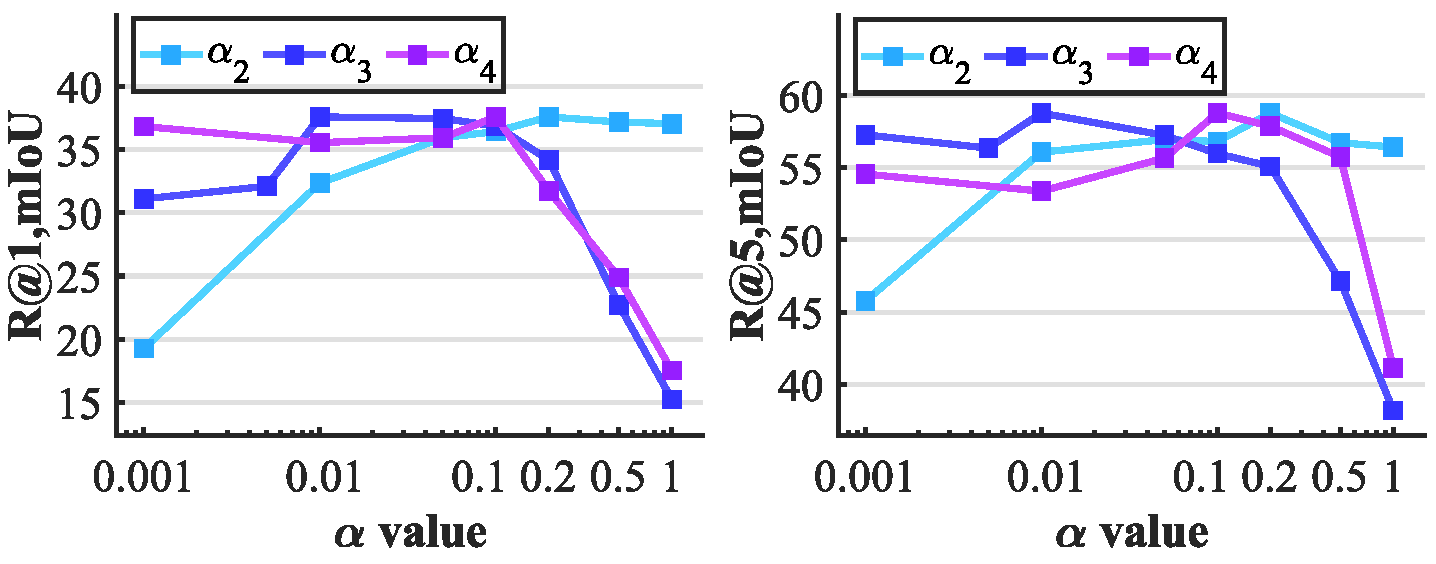
\includegraphics[width=\linewidth]{figures/3-ablation-graph-alpha.pdf}
    \caption{Ablation studies by varying $\alpha$ values for the pull-push learning scheme on the ActivityNet Captions dataset.
    }
    \label{fig:ablation-graph-alpha}
\end{figure}

%% Qualitative Results %%%%%%%%%%%%%%%%%%%%%%%%%%%%%%
\subsection{Qualitative Results}
\label{sec:qualitative-results}
%%%%%%%%%%%%%%%%%%%%%%%%%%%%%%%%%%%%%%%%%%%%%%%%%%%%%%%%%%%%

\cref{fig:qualitative} shows qualitative results of our PPS and other variants of PPS.
It is notable that PPS captures accurate query-relevant locations, while the ground truth, which can be noisy due to the subjectivity of annotators, includes redundant locations such as a logo at the beginning of the video.
% More qualitative results for the visualization of proposals are shown in Supplementary material.


\begin{figure}[t]
  \centering
  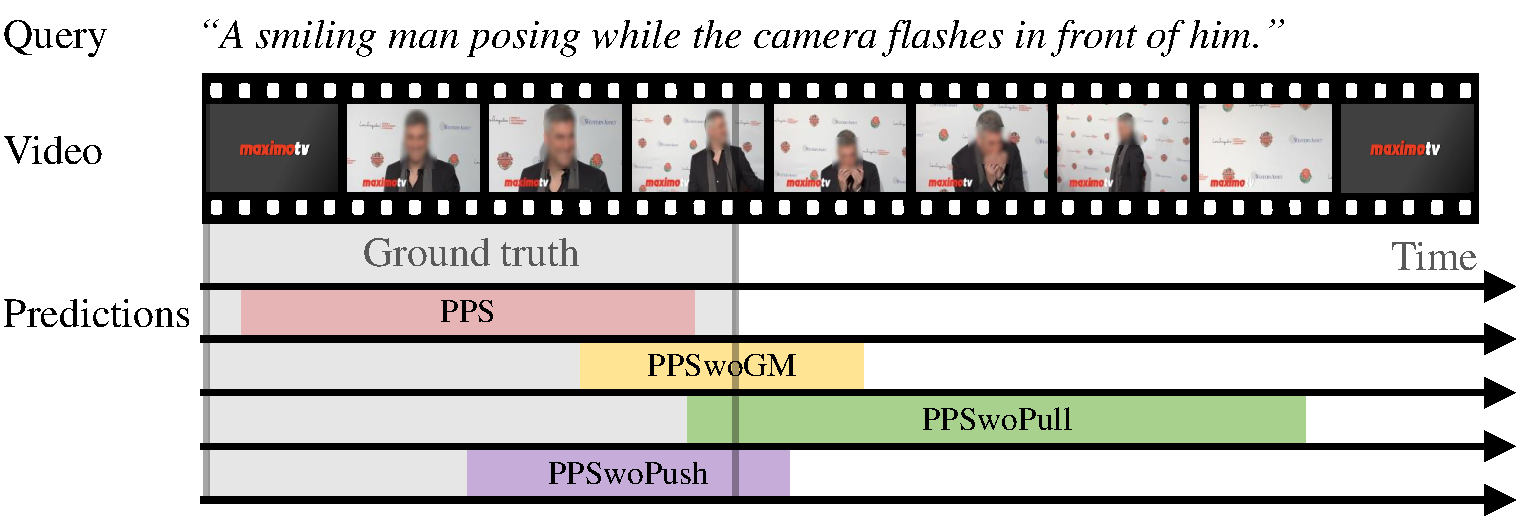
\includegraphics[width=\linewidth]{figures/4-qualitative.pdf}
  \caption{
  Qualitative results on the Activity-Net Captions dataset.
  Given a video and a query, PPS yields a predicted temporal location (red).
  We also visualize the predictions of variants using a positive proposal of one Gaussian mask without the mixture (yellow) or excluding a pulling loss (green) or excluding pushing losses (purple).
  }
\label{fig:qualitative}
\end{figure}

\section{Conclusion}
\section{Conclusion}
In this work, we adapted two state-of-the-art CSSL frameworks, CaSSLe and Kaizen, from visual representation learning to human activity recognition, one of the fundamental tasks in human-centric computing. Our evaluation indicates that a unified training scheme handling both representation learning and classification learning, as proposed in Kaizen, can perform better under realistic data assumptions, with the advantage of being deployable at any point during the process, which is particularly vital for HAR and other human-centric applications. Additional experiments indicate that the use of a progressive importance coefficient which adaptively adjusts the importance of knowledge retention and classification learning can allow us to explore the trade-off between different learning objectives, reaching higher levels of performance compared to a fixed loss function. This work demonstrated the potential of utilising self-supervised learning for developing human activity recognition models that can adapt to changes in user behaviours.


\section*{Acknowledgments}
This work was supported by IITP grant funded by Korea government(MSIT) [No.B0101-15-0266, Development of High Performance Visual BigData Discovery Platform for Large-Scale Realtime Data Analysis; NO.2021-0-01343, Artificial Intelligence Graduate School Program (Seoul National University)] and the BK21 FOUR program of the Education and Research Program for Future ICT Pioneers, Seoul National University in 2023.


%-------------------------------------------------------------------------

%%%%%%%%% REFERENCES
\bibliography{aaai24}


%%%%%%%%% Supplementary materials
% \input{7-supplementary}

\end{document}

